\documentclass[12pt]{report}

\usepackage[margin=1.0in]{geometry}
\usepackage{fancyhdr}
\usepackage{hyperref}

\usepackage{graphicx}

\pagestyle{fancy}

\lhead{Rook: Implementation Details}
\rhead{Nathan Esau}

\begin{document}

\tableofcontents

\chapter{Introduction}

\section{Existing Implementations}

An implementation of the Rook Game can be found at \url{https://sites.google.com/site/btsoftwarehomepage/Home/Rook}. Note that the source code for this version is not available.

A screenshot of this version of the game is shown in Figure \ref{fig:taylorproductionsrook}.

\begin{figure}[ht]
\caption{Screenshot of Rook game by Taylor Productions}
\label{fig:taylorproductionsrook}
\begin{center}
\includegraphics[width=0.6\textwidth]{images/TaylorProductionsRook}
\end{center}
\end{figure}

\chapter{\texttt{Rook}: Implementation Details}

\section{Algorithms}

\subsection{Starting the Game}

The start of the Rook game is implemented in \texttt{GameController::StartGame}. The sequence is

\begin{enumerate}
\item Initialize Card Deck
\item Shuffle Card Deck
\item Deal Card Deck to Players
\item Display Cards
\end{enumerate}

\section{Global Variables}

The global variables are shown in Table \ref{tab:globalvariables}.

\begin{table}[ht]
\centering
\begin{tabular}{l l}
\hline
Variable & Description \\ \hline
\texttt{GUI *gui} & Access to interface throughout code \\ \hline
\texttt{GameController *gc} & Event handlers need to be able to access \texttt{gc} \\ \hline
\end{tabular}
\caption{Global variables}
\label{tab:globalvariables}
\end{table}

\chapter{User Guide}

\section{Introduction}

Rook is a card game played with partners that was originally created by Parker Bros in 1906. It uses a specialized deck of cards. The deck is made up of 57 cards and split into four main suits. The main suits are Black, Red, Green, and Yellow. Each of the suits consists of the cards 1--14. An additional wild card called the rook is also part of the deck. The rook card is shown in Figure \ref{fig:rookcard}.

\begin{figure}[ht]
\caption{Rook card}
\label{fig:rookcard}
\begin{center}
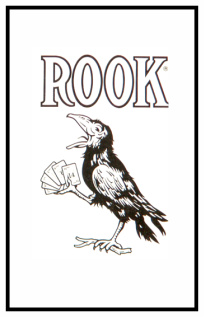
\includegraphics[width=0.25\textwidth]{images/rook}
\end{center}
\end{figure}

\section{Rules}

Rook is a ``Trick'' taking game. A Round/Trick consists of each player playing one card. The card of greatest value ``takes the trick'' and wins all cards played that round for their team. The player who wins a round also leads in the next round. Players must follow suit whenever possible. If a player is unable to follow suit then they have the opportunity to trump in or throw off. There are 120 points available in the rook deck. The object of the game is to win as many of the 120 possible points for your team in each hand. At the end of each hand, the teams add up the points acquired and they see if the team who the bid matched or exceeded their bid. If the team who won the bid did not make their bid then they are ``set''. When a team is set, the team's bid value is subtracted from their total score. Otherwise, each team adds the points won in that hand to their total score. The first team to reach the winning score wins the game.

\section{Point Cards}

A list of cards and their point values is shown in Table \ref{tab:pointcards}.

\begin{table}[ht]
\begin{center}
\begin{tabular}{l r}
Card & Point Value \\ \hline
5's of all suits & 5 \\
10's of all suits & 10 \\
14's of all suits & 10 \\
Rook & 20 \\ \hline
\end{tabular}
\end{center}
\caption{Point values for Rook Cards}
\label{tab:pointcards}
\end{table}

\section{Bidding}

The player who deals starts bidding. Bidding is done in increments of 5 points and goes clockwise in direction. Bidding continues until all but one player has passed or a player bids 120 points. When a player wins the bid, they must choose a trump suit. After choosing the trump suit, the kitty card is added to the bid winner's hand and the player must choose a card to discard. The player may discard any card that is not worth points. It is inadvisable to discard any cards of the trump suit.

\section{Scoring}

After each round has been played, the cards are scored and the team who played the card of highest value wins all cards played that round. If trump was played then the highest rank trump played is the winning card. Otherwise, the highest ranked card that is the same suit as the suit lead wins the round.

\section{Glossary}

A list of game words is shown in Table \ref{tab:glossaryterms}.

\begin{table}[ht]
\begin{center}
\begin{tabular}{l p{10cm}}
\hline
Term & Definition \\ \hline
Round/ Trick & Each player playing one card \\ \hline
Hand & Playing rounds until all cards have been played \\ \hline
Kitty Card & The extra card left after dealing cards to the players. This card is given to the player who wins the bid \\ \hline
Trump Suit & The suit that the bid winners chooses to be trump. The trump suit is more valuable than any other suit. Even a low ranked trump is more powerful than a high ranked non-trump. \\ \hline
Discard & The card removed from a players hand after they win the bid, select a trump suit, and the kitty card is mixed into their hand. The discarded card must not be worth points. \\ \hline
Bid Value & The value a player has bid \\ \hline
Rook Card & The wild card that becomes the highest trump card and therefore the most powerful card. \\ \hline
\end{tabular}
\end{center}
\caption{Glossary of terms}
\label{tab:glossaryterms}
\end{table}


\end{document}